\chapter{QUANTUM NATURAL LANGUAGE PROCESSING (QNLP)}
\hspace*{0.3in}Quantum Natural Language Processing (QNLP) is an emerging area of Quantum Artificial Intelligence that explores how quantum mechanics can enhance the way machines understand and process human language. Three main paradigms dominate current research: distributional models, which represent word meanings as high-dimensional vectors encoded in quantum states; compositional models, such as the distributional compositional categorical (DisCoCat) framework, which map grammatical structures into quantum circuits for syntactic-semantic alignment; and hybrid models that integrate classical NLP with quantum subroutines to balance scalability with near-term quantum hardware constraints. Early applications of QNLP include semantic similarity detection, question answering, and low-resource machine translation, where the parallelism of quantum states provides richer contextual representations [7].\\
\begin{figure}[htbp]
	\centering
	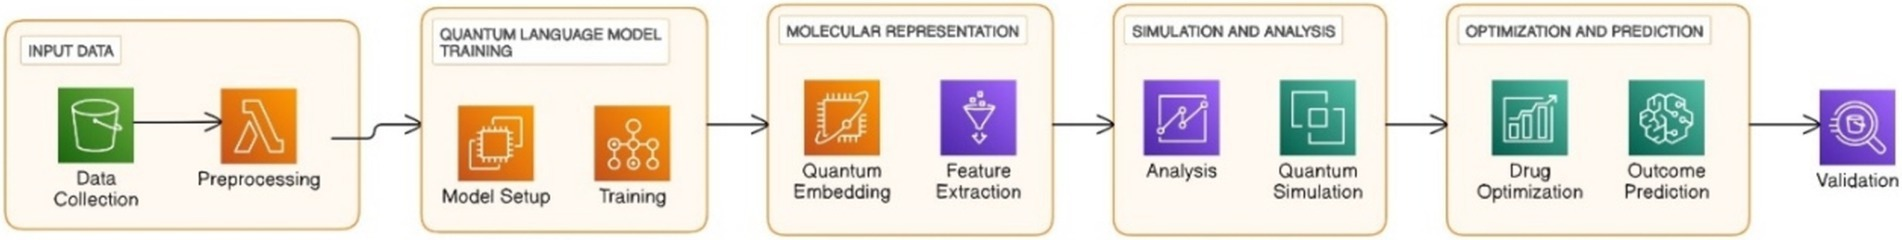
\includegraphics[width=1\linewidth]{qnlpD.jpg}
	\caption{QNLP drug discovery and design.}
	\label{fig:enter-label}
\end{figure}
\\
\begin{figure}[htbp]
	\centering
	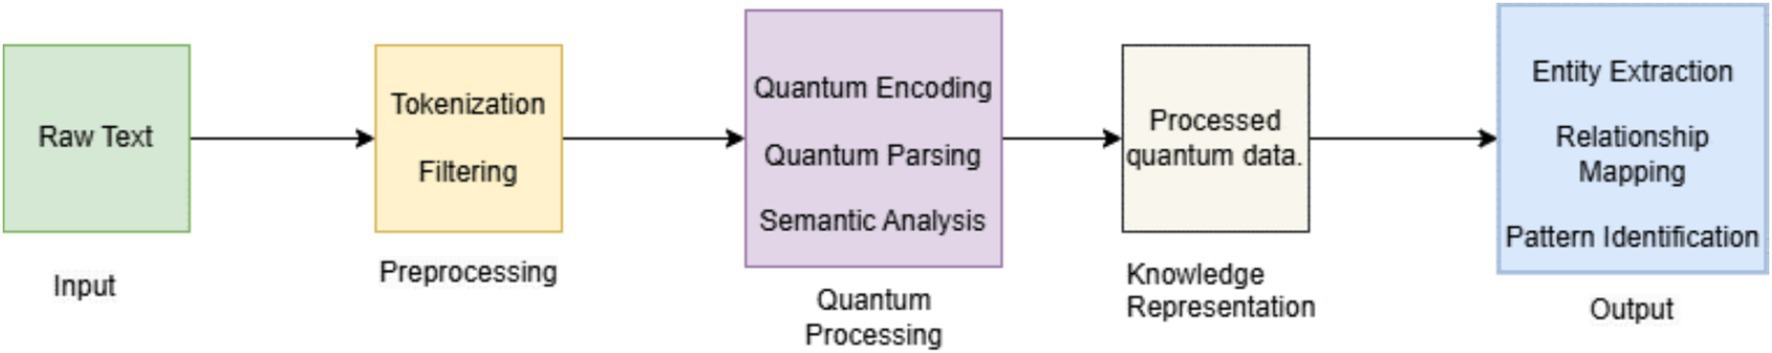
\includegraphics[width=1\linewidth]{qnlpG.jpg}
	\caption{QNLP literature mining and knowledge extraction.}
	\label{fig:enter-label}
\end{figure}
\\
\hspace*{0.3in}Despite this promise, today’s noisy intermediate-scale quantum (NISQ) devices face major limitations, including noise, decoherence, and limited qubit counts, restricting QNLP to smaller tasks rather than large-language-model (LLM)-scale workloads. The roadmap toward practical QNLP requires algorithmic innovation in quantum embeddings and DisCoCat circuits, hardware advances in error-corrected and modular qubits, and hybrid integration where quantum accelerates specific language subtasks while classical systems manage scale. By 2029, QNLP is expected to serve as a complementary layer to classical LLMs, augmenting semantic reasoning, disambiguation, and symbolic integration rather than replacing established large-scale models [8].
